\chapter{Background}\label{chap.background}
\minitoc


%%%%%%%%%%%%%%%%%%%%%%%%
\section{Introduction}
In today's digital age, artificial intelligence (AI) has established itself as a transformative force, permeating virtually every facet of our lives, from healthcare diagnostics to real-time language translation, and from autonomous vehicles to personalized content recommendations. At the heart of this AI revolution lie neural networks-computational models inspired by the human brain's intricate web of neurons. These algorithms have demonstrated an unparalleled ability to discern patterns, extract insights, and make predictions from vast swathes of data, often matching or even surpassing human capabilities in certain domains.

However, the explosive growth and complexity of neural networks have also ushered in significant computational challenges. Deep neural networks, characterized by their multi-layered architectures, can contain millions, if not billions, of parameters. Training and deploying these behemoths demand staggering amounts of computational power. Traditional Central Processing Units (CPUs), while versatile, are not inherently optimized for the parallel and matrix-based computations that neural networks frequently rely upon. This computational bottleneck not only impacts the speed and efficiency of neural network operations but also their energy consumption a critical concern in our increasingly mobile and interconnected world.

Enter hardware accelerators, specialized hardware designed to expedite specific computations. For neural networks, accelerators like Graphics Processing Units (GPUs) and Tensor Processing Units (TPUs) have emerged as pivotal players, providing the much-needed horsepower to drive neural computations swiftly and efficiently. Yet, as the quest for speed and efficiency continues, there's a growing interest in further refining these accelerators, particularly through custom numerical representations such as custom floating-point computation. This avenue promises a harmonious blend of performance and power efficiency, potentially heralding a new era for neural network hardware.

In this chapter, we delve into the intricate world of neural networks, their indelible mark on modern computation, and the imperatives driving the development of dedicated hardware accelerators. Through this exploration, we set the stage for our deep dive into low-power neural network accelerators leveraging custom floating-point computation a frontier at the nexus of AI's potential and practicality.

\section{Neural Networks: Fundamentals}

\subsection{Architecture}
A neural network is composed of layers of interconnected nodes or neurons. The complexity and depth of the architecture can vary, but the fundamental structure consists of:
\begin{itemize}
	\item \textbf{Input Layer}: The initial layer where data is fed into the network.
	\item \textbf{Hidden Layers}: Layers that lie between the input and output. These layers process and transform input data.
	\item \textbf{Output Layer}: The final layer where the network produces its predictions or classifications.
\end{itemize}

\subsection{Nodes (Neurons)}
\begin{description}
	\item[Definition] A node (or neuron) is a fundamental computational unit of a neural network. It receives one or more inputs, processes them, and produces an output.
	\item[Components]
	
	\begin{itemize}
		\item \textbf{Input}: Values from previous layers or data inputs.
		\item \textbf{Transfer Function}: Combines the inputs, often in a weighted sum.
		\item \textbf{Activation Function}: Transforms the result of the transfer function into the neuron's output.
	\end{itemize}
\end{description}

\subsection{Layers in a Neural Network}
\begin{description}
	\item[Input Layer] Receives raw data inputs. The number of nodes here often corresponds to the number of input features.
	\item[Hidden Layers] These layers aren't directly exposed to either the raw input or final output. They capture and process complex patterns in the data. Deep Neural Networks (DNNs) have many hidden layers.
	\item[Output Layer] The predictions or classifications are formed here. The number of nodes typically matches the number of desired outputs, like categories in a classification task.
\end{description}

\subsection{Weights and Biases}
\begin{description}
	\item[Weights] These represent the strength or intensity of the connection between two neurons. They scale the data as it flows through the network. During training, these weights are adjusted to minimize the difference between the predicted output and the actual target values.
	\item[Biases] Bias is an additional parameter in the neuron that enables it to produce outputs even when all its inputs might be zero. Think of it as an offset or intercept. Like weights, biases are adjusted during training to optimize network performance.
\end{description}

\subsection{Activation Functions}
The activation function is critical to introducing non-linear properties into the network, allowing it to learn from error and make adjustments, essential for learning complex patterns.
\begin{description}
	\item[Sigmoid] Maps any input to a value between 0 and 1, making it useful for binary classification. Its equation is:
	\begin{equation}
	f(x) = \frac{1}{1 + e^{-x}}
	\end{equation}
	\item[Tanh (Hyperbolic Tangent)] Similar to sigmoid but maps values to a range between -1 and 1. Its equation is:
	\begin{equation}
	f(x) = \frac{e^{x} - e^{-x}}{e^{x} + e^{-x}}
	\end{equation}
	\item[ReLU (Rectified Linear Unit)] It replaces all negative values with zero and has become a default choice for many types of neural networks because it often leads to faster convergence during training. Its equation is:
	\begin{equation}
	f(x) = \max(0, x)
	\end{equation}
	\item[Softmax] Often used in the output layer of a classification network, it converts raw score outputs into a probability distribution across multiple classes.
\end{description}

Neural networks, with their layers, nodes, weights, biases, and activations, form a flexible and potent framework capable of learning and representing complex patterns and functions. Their ability to adapt and learn from data makes them a cornerstone of modern artificial intelligence applications.


\section{Evolution of Neural Networks}

\subsection{Perceptrons}

Introduced by Frank Rosenblatt in the 1950s, the perceptron can be viewed as a single-layer neural network:
\[ y = f(\mathbf{w} \cdot \mathbf{x} + b) \]
where:
\begin{itemize}
	\item \( y \) is the output.
	\item \( \mathbf{w} \) is the weight vector.
	\item \( \mathbf{x} \) is the input vector.
	\item \( b \) is the bias.
	\item \( f \) is a step function.
\end{itemize}

\subsection{Multi-layer Perceptrons (MLP)}

MLPs are extensions of perceptrons with one or more hidden layers. The output of each layer is computed as:
\[ \mathbf{h}^{(l)} = f(\mathbf{W}^{(l)} \mathbf{h}^{(l-1)} + \mathbf{b}^{(l)}) \]
for \( l = 1, \ldots, L \), where \( L \) is the number of layers, and \( f \) is an activation function (e.g., sigmoid or tanh).

The backpropagation algorithm adjusts the weights using:
\[ \frac{\partial E}{\partial \mathbf{w}_{ij}} = -(t_i - y_i) f'(h_j) x_j \]
where \( E \) is the error, \( t_i \) is the target, and \( y_i \) is the network's output.

\subsection{Deep Neural Networks (DNNs)}

DNNs are MLPs with a large number of layers. The computation for each layer remains as in MLPs, but DNNs often incorporate more advanced activation functions like ReLU:
\[ f(x) = \max(0, x) \]

\subsection{Convolutional Neural Networks (CNNs)}

CNNs are specialized for spatial hierarchies in data. For a convolutional layer:
\[ \mathbf{h}_{i,j}^{(l)} = f\left( \sum_{m,n} \mathbf{W}^{(l)}_{m,n} \cdot \mathbf{h}_{i+m,j+n}^{(l-1)} + b^{(l)} \right) \]
where:
\begin{itemize}
	\item \( \mathbf{h}_{i,j}^{(l)} \) is the output at position \( (i,j) \) in layer \( l \).
	\item \( \mathbf{W}^{(l)}_{m,n} \) is the kernel at offset \( (m,n) \) in layer \( l \).
\end{itemize}



\section{Motivation: The Limitations of CPUs for Neural Network Processing}

Neural networks, particularly deep learning models, have emerged as powerful tools for a variety of complex tasks ranging from computer vision to natural language processing. As these networks grow in depth and complexity, their computational and memory demands intensify, thereby revealing the inherent limitations of traditional computing architectures.

\subsection{Parallelism}

\textbf{Challenge}: Neural network computations, especially in the training phase, require numerous parallel operations like matrix multiplications. CPUs, with their limited core counts, aren't inherently designed to handle such vast parallelism efficiently.

\textbf{Implication}: Training a deep neural network on a CPU can be prohibitively slow, especially when dealing with large datasets.

\subsection{Memory Bottlenecks}

\textbf{Challenge}: The iterative nature of neural network training often requires frequent data transfers between the CPU and main memory. This can lead to memory bottlenecks, given the hierarchical memory structure and bandwidth limits associated with CPUs.

\textbf{Implication}: The performance of neural network models can be severely hampered by these memory bottlenecks, leading to longer training times.

\subsection{Energy Efficiency}

\textbf{Challenge}: CPUs, being general-purpose processors, are not optimized for the specific operations that dominate neural network computations. This lack of specialization can lead to inefficient power consumption.

\textbf{Implication}: Training or inferencing on CPUs can be energy-inefficient, which is especially problematic for mobile devices or other power-constrained environments.

\subsection{Flexibility vs. Specialization}

\textbf{Challenge}: While CPUs are designed to be general-purpose and flexible, neural network processing often benefits from specialized hardware that can accelerate specific operations.

\textbf{Implication}: CPUs may not offer the best trade-off between flexibility and performance for neural network applications. Specialized hardware like GPUs, TPUs, and custom ASICs often provide significant speedups.

The exponential growth in the scale and complexity of neural network models necessitates a rethinking of traditional computational approaches. While CPUs remain indispensable in the broader landscape of computing, specialized architectures are increasingly becoming the go-to choice for neural network processing due to their performance, efficiency, and scalability advantages.


\section{Overview of Hardware Accelerators for Neural Network Processing}

\subsection{Graphics Processing Units (GPUs)}

\textbf{Introduction}: Initially designed for rendering graphics, GPUs have been repurposed for parallel computations due to their vast number of cores.

\textbf{Benefits}:
\begin{itemize}
	\item Massively parallel architecture: Suitable for matrix operations in neural networks.
	\item General-purpose: Flexible enough for various computational tasks beyond graphics.
\end{itemize}

\textbf{Challenges}:
\begin{itemize}
	\item Power consumption can be high under load.
	\item Memory bandwidth can become a bottleneck for very large models.
\end{itemize}

\textbf{Key Mathematical Insight}:
\[ \text{Speedup} = \frac{\text{Serial Execution Time}}{\text{Parallel Execution Time}} \]

\subsection{Field-Programmable Gate Arrays (FPGAs)}

\textbf{Introduction}: FPGAs are reconfigurable integrated circuits, enabling hardware-level customizations.

\textbf{Benefits}:
\begin{itemize}
	\item Customizable: Can be tailored for specific tasks.
	\item Power-efficient: Can be optimized for energy efficiency.
\end{itemize}

\textbf{Challenges}:
\begin{itemize}
	\item Steeper learning curve: Requires hardware description language knowledge.
	\item Less performance compared to ASICs for specific tasks due to their general-purpose nature.
\end{itemize}

\textbf{Key Mathematical Insight}:
\[ \text{Frequency} = \frac{1}{\text{Propagation Delay}} \]

\subsection{Application-Specific Integrated Circuits (ASICs)}

\textbf{Introduction}: ASICs are optimized for a specific application, enhancing performance and efficiency for that task.

\textbf{Benefits}:
\begin{itemize}
	\item Peak Performance: Designed specifically for a task.
	\item Energy Efficiency: Less power consumption due to specialized architecture.
\end{itemize}

\textbf{Challenges}:
\begin{itemize}
	\item Inflexible: Cannot be repurposed for other tasks.
	\item High initial development cost and time.
\end{itemize}

\textbf{Key Mathematical Insight}:
\[ \text{Power Consumption} \propto \text{Capacitive Load} \times \text{Voltage}^2 \times \text{Frequency} \]

\subsection{Tensor Processing Units (TPUs)}

\textbf{Introduction}: Designed by Google, TPUs are tailored for tensor computations in machine learning tasks.

\textbf{Benefits}:
\begin{itemize}
	\item High Throughput: Designed for large-scale matrix operations.
	\item Efficient: Optimized for specific tensor computations, leading to energy savings.
\end{itemize}

\textbf{Challenges}:
\begin{itemize}
	\item Less flexible compared to GPUs: Primarily tailored for tensor computations.
	\item Accessibility: Not as commonly available as GPUs for individual developers.
\end{itemize}

\textbf{Key Mathematical Insight}:
\[ \text{Matrix Multiplier Throughput} = \text{Number of MAC units} \times \text{Frequency} \]

As neural network processing demands grow, a spectrum of hardware accelerators has emerged, each with its strengths and trade-offs. The choice of accelerator hinges on the task's specific requirements, including performance, power, flexibility, and cost.


\section{The Quest for Low-Power Neural Computing}

In the modern era of ubiquitous computing, power efficiency has emerged as a pivotal factor shaping the design, operation, and environmental impact of electronic devices. From individual user experiences with mobile devices to the colossal operational demands of data centers, efficient power management plays a decisive role. This discussion elucidates the significance of power efficiency, underpinned by relevant equations.


Power efficiency weaves its way into the fabric of our digital society, having far-reaching implications on usability, economic viability, and environmental sustainability. Mathematical modeling and understanding of power dynamics can guide better decision-making in both device design and infrastructure management.

\subsection{Power Reduction Techniques in Neural Network Accelerators}

The rapid surge of deep learning models, particularly neural networks, has necessitated the deployment of specialized hardware accelerators to meet computational demands. As these models find applications in mobile and embedded systems, power efficiency becomes paramount. This section explores key techniques such as approximate computing, quantization, and custom floating-point computation, tailored to optimize the power footprint in neural network accelerators.

\subsubsection{Approximate Computing}

\textbf{Definition:} Approximate computing is a paradigm wherein certain computations are allowed to be inexact to save power or improve performance.

\textbf{Explanation:} Neural networks, by their nature, exhibit resilience to errors due to their redundant structures. Leveraging this, certain arithmetic operations within the network can be performed approximately, without significant degradation in output quality. 

\textbf{Supporting Equations:}
Assuming power consumption is proportionally related to the precision of computation, we can express:
\begin{equation}
P_{\text{approx}} = \alpha P_{\text{exact}}
\end{equation}
Where \( P_{\text{exact}} \) is the power consumption with exact computing, \( P_{\text{approx}} \) is with approximate computing, and \( 0 \leq \alpha \leq 1 \) represents approximation efficiency.

\subsubsection{Quantization}

\textbf{Definition:} Quantization refers to the process of constraining input values from a large set to output in a smaller set.

\textbf{Explanation:} Neural network weights and activations, traditionally stored in floating-point format, can be quantized to a fixed-point or even lower bit-width representation. This drastically reduces both memory footprint and computation energy. Post-training quantization and training-time quantization are methodologies that ensure minimal accuracy loss post this bit-width reduction.

\textbf{Supporting Equations:}
For a uniform quantizer, quantization error \( \Delta \) for an \( N \)-bit representation is:
\begin{equation}
\Delta \approx \frac{\text{Full Scale Range}}{2^N}
\end{equation}

Furthermore, assuming energy scales with the square of bit width (primarily due to the quadratic scaling of digital multiplication energy with operand width):
\begin{equation}
E_{\text{quantized}} = \left( \frac{N_{\text{quantized}}}{N_{\text{full}}}\right)^2 E_{\text{full}}
\end{equation}

\subsubsection{Custom Floating-Point Computation}

\textbf{Definition:} Custom floating-point computation involves modifying traditional IEEE 754 floating-point standards to meet specific power, area, or accuracy requirements.

\textbf{Explanation:} Neural network computations often don't require the entire dynamic range or precision offered by standard floating-point formats. By customizing the bit-widths of the exponent and mantissa fields, or by using block floating-point formats where multiple values share a common exponent, significant power savings can be achieved.

\textbf{Supporting Equations:}
IEEE 754 floating-point representation is:
\begin{equation}
F = (-1)^{\text{sign}} \times (1.\text{mantissa}) \times 2^{\text{exponent} - \text{bias}}
\end{equation}

Power reduction from bit-width customization can be conceptualized as:
\begin{equation}
P_{\text{custom}} = \beta P_{\text{IEEE}}
\end{equation}
Where \( P_{\text{IEEE}} \) is the power using standard IEEE formats, \( P_{\text{custom}} \) is with custom floating-point, and \( 0 \leq \beta \leq 1 \) is an efficiency parameter.

Conclusively, while the aforementioned techniques offer compelling advantages in power reduction, it's imperative to holistically evaluate their impact on the overall accuracy and performance of neural network accelerators. Future work in this realm will undoubtedly aim at striking an optimal balance between power savings and computation fidelity.

\subsection{Relationship Between Computational Precision and Power Consumption}

\textbf{Definition:} Computational precision refers to the number of bits used to represent and process data. Power consumption, particularly in digital hardware like arithmetic units and memory, scales with the bit-width of the data.

\textbf{Explanation:} The relationship between precision and power stems from multiple factors:

\begin{itemize}
	\item \textbf{Dynamic Power:} Every bit operation, like addition or multiplication, consumes dynamic power. As the bit-width increases, the number of transistors switching (and thus, dynamic power) increases.
	
	\item \textbf{Static Power:} More bits mean larger circuits, which in turn increases the total silicon area and static (or leakage) power.
	
	\item \textbf{Memory Access Power:} Higher precision requires more storage, leading to increased memory access power. This includes both reading from memory and writing to memory.
\end{itemize}

\textbf{Supporting Equations:}
Let's assume that the power consumed is directly proportional to the square of the bit-width (due to quadratic scaling of multiplication energy and increased area). If \( P_b \) is the power for a computation with \( b \) bits of precision and \( P_{b'} \) is the power for \( b' \) bits of precision, then the relationship can be expressed as:

\begin{equation}
\frac{P_b}{P_{b'}} = \left(\frac{b}{b'}\right)^2
\end{equation}

This equation suggests that if we double the precision, the power consumption could increase by a factor of four (assuming other factors remain constant). However, this is a simplified representation, and in real systems, other factors, such as the efficiency of the hardware design, also play a crucial role.

The relationship between computational precision and power consumption is pivotal in the context of neural network accelerators. Precision reduction, without significantly affecting the model's accuracy, can lead to substantial power savings. This insight guides the exploration of techniques like approximate computing, quantization, and custom floating-point formats.


\section{IEEE Standard for Floating-Point Arithmetic}

The IEEE 754 standard is a technical standard for floating-point computation, established in 1985 by the Institute of Electrical and Electronics Engineers (IEEE). Over the years, it has become the most widely used standard for floating-point computation in computer systems.

\subsection{Structure of IEEE 754 Representation}

The IEEE 754 standard defines both single-precision (32-bit) and double-precision (64-bit) formats, among others. The components of these representations include:

\begin{itemize}
	\item \textbf{Sign bit (S):} One bit representing the sign of the number. \(0\) for positive and \(1\) for negative.
	\item \textbf{Exponent (E):} Represents the power of two to which the number is raised. The exponent is biased in the standard representation.
	\item \textbf{Fraction (F) or Mantissa:} Represents the actual digits of the number.
\end{itemize}

For single precision:
\begin{itemize}
	\item Sign bit: 1 bit
	\item Exponent: 8 bits
	\item Fraction: 23 bits
\end{itemize}

For double precision:
\begin{itemize}
	\item Sign bit: 1 bit
	\item Exponent: 11 bits
	\item Fraction: 52 bits
\end{itemize}

The value \(V\) of an IEEE 754 number is given by:
\begin{equation}
V = (-1)^S \times (1 + F) \times 2^{(E - \text{bias})}
\end{equation}
Where bias is \(127\) for single-precision and \(1023\) for double-precision.

\subsection{Benefits of IEEE 754 Standard}

\begin{itemize}
	\item \textbf{Uniformity:} Provides a standard across different computing platforms ensuring portability of code.
	\item \textbf{Wide Range:} The floating-point representation allows for a vast range of numbers, from extremely small to very large values.
	\item \textbf{Special Values:} Represents not just normalized numbers but also denormalized numbers, NaN (Not a Number), infinities, and zero.
	\item \textbf{Rounding and Precision:} Defines rules for rounding, ensuring accuracy in arithmetic operations.
\end{itemize}

\subsection{Limitations of IEEE 754 Standard}

\begin{itemize}
	\item \textbf{Inexact Representation:} Not all real numbers can be exactly represented, leading to rounding errors.
	\item \textbf{Floating-Point Errors:} Operations can lead to issues like overflow, underflow, and precision errors.
	\item \textbf{Complex Hardware:} Implementing IEEE 754 compliant FPU (Floating Point Units) can be hardware-intensive.
	\item \textbf{Inconsistencies:} Due to issues like NaN not being equal to itself, certain comparisons and operations can lead to unexpected results.
\end{itemize}

While the IEEE 754 standard has been instrumental in unifying floating-point arithmetic across platforms, it is essential for developers and hardware designers to understand its intricacies and potential pitfalls. Especially in critical applications, the nuances of floating-point arithmetic under this standard must be carefully managed to ensure correctness and reliability.

\section{Errors and Limitations in Floating-Point Computation}

Floating-point computation, while powerful, is subject to several errors and limitations due to its discrete nature. These errors might seem minuscule for individual operations but can compound in iterative processes or in scenarios where precision is paramount, such as neural networks.

\subsection{Types of Floating-Point Errors}

\begin{itemize}
	\item \textbf{Rounding Errors:} Since floating-point representation can only approximate real numbers with a finite number of bits, many numbers are rounded to the nearest representable number.
	
	\item \textbf{Truncation Errors:} These occur when numbers with more precision than the format can handle are truncated.
	
	\item \textbf{Overflow and Underflow:} Overflow happens when a number is too large to be represented in the floating-point format. Conversely, underflow occurs when a number is too close to zero for the format to represent.
	
	\item \textbf{Loss of Significance:} It occurs when performing operations on numbers with widely differing magnitudes. Subtracting two nearly equal floating-point numbers can lead to significant precision loss.
	
	\item \textbf{Catastrophic Cancellation:} This happens when two nearly equal numbers are subtracted, yielding a result that lacks significant digits of precision.
\end{itemize}

\subsection{Implications in Neural Networks}

Neural networks involve vast amounts of matrix multiplications, nonlinear activations, and iterative optimization processes, making them sensitive to the aforementioned errors.

\begin{itemize}
	\item \textbf{Weight Degradation:} Small errors in computation can gradually modify the weights, which over several iterations, can cause the model to deviate from its optimal configuration.
	
	\item \textbf{Loss Divergence:} Especially in deep networks, small errors can be amplified across layers, causing the loss function to diverge.
	
	\item \textbf{Activation Saturation:} Rounding or truncation errors can push activations into saturated regions of activation functions (like the sigmoid), causing the gradient to vanish.
	
	\item \textbf{Training Instability:} Floating-point errors can introduce instability during training, making it challenging to achieve convergence.
	
	\item \textbf{Generalization Issues:} Errors in representation can lead to a neural network overfitting to the training data, reducing its ability to generalize well on unseen data.
\end{itemize}

\section{Traditional Floating-Point Formats for Neural Networks}

Deep learning and neural network models have exhibited tremendous success across various domains, from image and speech recognition to natural language processing. However, the computational demands of training and deploying these models are immense. As a result, hardware accelerators, custom architectures, and specialized numerical formats are actively researched to enhance performance and efficiency. Within this context, the appropriateness of conventional floating-point representations comes under scrutiny.

\subsection{Inherent Inefficiencies}

\begin{itemize}
	\item \textbf{Over-precision:} Neural networks have showcased remarkable resilience to noise and quantization. Often, the high precision offered by traditional floating-point formats like double or even single precision is unnecessary, leading to wasted computational and memory resources.
	
	\item \textbf{Dynamic Range Overhead:} While the broad dynamic range of floating-point numbers is beneficial for many scientific computations, neural networks, especially once trained, usually operate within a more constrained range. This means that the wide range offered by standard formats may be overkill, again wasting resources.
\end{itemize}

\subsection{Power and Area Costs}

The silicon area and power consumption associated with floating-point units (FPUs) that support traditional formats are significantly higher than their fixed-point or lower-precision counterparts.

\begin{itemize}
	\item \textbf{Complex Arithmetic Units:} Floating-point addition, multiplication, and especially division are complex operations, demanding a larger silicon footprint and increased power consumption.
	
	\item \textbf{Storage Overheads:} Storing weights, activations, and gradients in high-precision formats increases memory demand and bandwidth requirements, leading to both area and energy inefficiencies.
\end{itemize}

\subsection{Latency Concerns}

The intricacy of floating-point operations can introduce latency, which is especially detrimental in real-time or edge deployments where swift responses are paramount.

\subsection{Customization Potential}

By moving away from standard floating-point formats, there's an opportunity to design custom numerical representations tailored to the specific requirements of neural networks. Such custom formats can be optimized for:

\begin{itemize}
	\item \textbf{Targeted Precision:} Match the precision to the specific tolerance of the neural network, ensuring computational efficiency without compromising accuracy.
	
	\item \textbf{Variable Dynamic Range:} Instead of a one-size-fits-all approach, the dynamic range can be adjusted based on the specific phase (e.g., training vs. inference) or layer of the neural network.
	
	\item \textbf{Hardware Efficiency:} Custom formats can be designed to simplify hardware implementations, reducing silicon area, power consumption, and potentially improving speed.
\end{itemize}

While traditional floating-point formats have served the computational world effectively for many applications, the peculiarities and tolerances of neural networks offer an opportunity. By reconsidering and potentially redefining numerical representations tailored to deep learning's unique demands, there's potential for significant improvements in efficiency, power, and performance.

\section{Custom Floating-Point Formats for Neural Network Computations}

Given the inefficiencies of traditional floating-point representations for neural network computations, several custom formats have been proposed to better suit the unique demands of deep learning applications. These formats aim to provide a balance between precision, dynamic range, and computational efficiency.


\subsection{Trade-offs of Custom Floating-Point Formats}

\begin{itemize}
	\item \textbf{Precision vs. Dynamic Range:} Custom formats often balance these two, optimizing for one sometimes at the cost of the other.
	\item \textbf{Performance vs. Accuracy:} Faster computations might be achieved at the expense of reduced accuracy or vice versa.
	\item \textbf{Complexity vs. Efficiency:} While some formats simplify hardware implementations, others might introduce complexities in certain operations.
	\item \textbf{Universality vs. Specialization:} Custom formats tailored for neural networks might not be optimal for other applications.
\end{itemize}

Custom floating-point formats hold significant promise for neural network computations by aligning the numerical representation's attributes with the specific demands of deep learning. However, selecting or designing an appropriate format requires a deep understanding of the inherent trade-offs and the specific requirements of the given application.


\section{State-of-the-Art Low-Power Neural Network Accelerators}

Neural network accelerators targeting low power are crucial for edge devices, wearables, and Internet-of-Things (IoT) devices. By optimizing power consumption, these accelerators enable complex neural network models to run on resource-constrained devices without depleting battery life.

\subsection{Accelerator Overview}

\begin{itemize}
	\item \textbf{Google Edge TPU:} A lightweight version of the Tensor Processing Unit (TPU) designed for edge devices. It is optimized for low latency and power efficiency for running TensorFlow Lite models.
	
	\item \textbf{NVIDIA Jetson Nano:} An embedded system-on-module (SoM) from NVIDIA, focusing on deploying machine learning models on edge devices with constrained power budgets.
	
	\item \textbf{Apple Neural Engine (ANE):} Part of the Apple A-series chips, ANE is designed for accelerating neural network computations in devices like iPhones, emphasizing both performance and power efficiency.
	
	\item \textbf{Intel Movidius Myriad X:} A vision processing unit (VPU) designed for running deep neural networks at the edge with an emphasis on low power and high performance.
\end{itemize}


\section{State-of-the-Art Low-Power Accelerators with Custom Floating-Point Formats}

In the race to achieve both power efficiency and computational precision, a new breed of accelerators has emerged. These designs utilize custom floating-point formats tailored to the nuances of neural network computations. This section reviews notable entries in this domain, emphasizing their approach to number representation and arithmetic.

\subsection{Accelerator Overview}

\begin{itemize}
	\item \textbf{Flexpoint Accelerators:} Dedicated hardware implementations optimized for the Flexpoint number format, which uses a shared exponent across a tensor to achieve a balance between precision and dynamic range.
	
	\item \textbf{Posit-Based Accelerators:} Hardware designs centered around the Posit number format, which provides more dynamic range and precision per bit than traditional IEEE floating-point formats.
	
	\item \textbf{Tapered FPUs:} Accelerators designed for the Tapered Floating-Point format, optimizing for scenarios where dynamic range is more crucial than precision.
\end{itemize}


Custom floating-point accelerators have brought a fresh perspective on achieving computational efficiency and precision. They challenge the status quo of traditional number representations, exploiting the unique properties of neural networks to achieve impressive performance in low-power scenarios.

\section{Gaps in Existing Solutions and Motivation for Further Exploration}

With the proliferation of deep neural networks in applications ranging from health diagnostics to autonomous vehicles, there's a surging demand for efficient, low-power accelerators. Despite significant advances in custom floating-point accelerators, several unresolved challenges remain that necessitate further research and innovation.

\subsection{Limitations of Current Approaches}

\begin{itemize}
	\item \textbf{Trade-off between Precision and Range:} While current custom formats address the dynamic range and precision issues to some extent, there's often a rigid trade-off. An optimal balance tailored for neural networks is still elusive.
	
	\item \textbf{Complex Arithmetic Operations:} Some custom floating-point formats introduce complicated arithmetic operations which can offset the gains made from using a reduced format in the first place.
	
	\item \textbf{Portability and Scalability:} Custom formats often lack widespread hardware and software support, making them less portable across various platforms. Their scalability to handle future, more complex neural network architectures is also untested.
	
	\item \textbf{Quantization Errors:} Reduced precision can sometimes lead to significant quantization errors. While neural networks are inherently robust, there's a limit to how much error can be introduced before accuracy degrades unacceptably.
\end{itemize}

\subsection{Need for Further Exploration}

Given the above challenges, there's a clear need to delve deeper into designing novel number representations and corresponding arithmetic operations that cater specifically to neural network requirements. Such research could lead to solutions that don't just retrofit existing number formats but truly synergize with the properties and tolerances of neural computations.

\subsection{Research Questions and Objectives}

In light of the identified gaps, this dissertation poses the following research questions:

\begin{enumerate}
	\item How can we design a floating-point format that optimally balances precision and dynamic range for neural network computations?
	\item What arithmetic operations can support this custom format to ensure both speed and accuracy?
	\item To what extent can the proposed format improve power efficiency without compromising the accuracy of neural network inferences and training?
\end{enumerate}

Consequently, the primary objectives of this research are:

\begin{itemize}
	\item To propose and formalize a novel reduced floating-point format tailored for neural networks.
	\item To design efficient arithmetic operations and hardware accelerators that leverage this format.
	\item To empirically validate the efficiency, speed, and accuracy of neural networks when using the proposed format, as compared to traditional and other custom floating-point formats.
\end{itemize}

By addressing these research questions and objectives, this dissertation aims to push the boundaries of what's currently achievable in low-power neural network accelerators. Through careful exploration and innovation, we aim to redefine the status quo, setting new benchmarks in both power efficiency and computational speed.


\section{Conclusion}

Over the course of this background chapter, we have journeyed through the evolution and intricacies of neural network accelerators, illuminating their critical function in today's AI-centric computational landscape. Beginning with the humble origins of neural acceleration and culminating in the advanced hardware constructs of today, we've seen that as computational demands evolve, so too do the tools and techniques crafted to meet them.

Neural networks, with their layers of complexity, have brought to the forefront the challenge of efficient computation. The need for power efficiency, especially in the context of embedded systems, adds another layer of complexity. The revelation that the IEEE standard floating-point representation, despite its ubiquity, might not be the paragon of efficiency for all neural computations has opened new frontiers of exploration. Enter custom floating-point formats, which promise to provide a unique blend of precision and efficiency tailored for the distinct requirements of neural networks.

As we pivot to the ensuing chapters, our lens will focus on the design methodologies geared towards Low-Power embedded systems. This exploration will delve deep into the architectures, trade-offs, and innovations that are shaping the next generation of power-efficient neural accelerators. 

With the foundational knowledge firmly established, it is time to navigate the intricate maze of low-power design, shedding light on strategies and techniques that could redefine the future of embedded neural computation.

\begin{quote}
	"In wisdom gathered over time, I have found that every experience is a form of exploration." - Ansel Adams
\end{quote}



%%%%%%%%%%%%%%%%%%%%%%%%


\section{Spike-by-Spike Neural Networks} 

\label{sec:sbs}

Technically, \gls{sbs} is a spiking neural network based on a
generative probabilistic model. It iteratively finds an estimate of
its input probability distribution $p(s)$ (i.e. the probability of
input node $s$ to stochastically send a spike) by its latent variables
via $r(s) = \sum_i h(i) W(s|i)$, 
where $\vec{h}$ is an inference
population composed of a group of neurons that compete with each
other. An \gls{ip_sbs} sees only the spikes $s_t$ (i.e. the
index identifying the input neuron $s$ which generated that spike at
time $t$ produced by its input neurons, not the underlying input
probability distribution $p(s)$ itself. By counting the spikes
arriving at a group of \gls{sbs} neurons, $p(s)$ is estimated by
$\hat{p}(s) = 1/T \sum_t \delta_{s,s^t}$ after $T$ spikes have been
observed in total. The goal is to generate an internal representation
$r(s)$ from the string of incoming spikes $s_t$ such that the negative
logarithm of the likelihood
$L = C - \sum_\mu \sum_s \hat{p}_\mu(s) log\left( r_\mu(s) \right)$ is
minimized. $C$ is a constant which is independent of the internal
representation $r_\mu(s)$ and $\mu$ denotes one input pattern from an
ensemble of input patterns. Applying a multiplicative gradient descent
method on $L$, an algorithm for iteratively updating $h_\mu(i)$ with
every observed input spike $s_t$ could be derived
\cite{ernst2007efficient}:
\begin{eqnarray} \label{eq:sbs_update}
h_\mu^{new}(i) = \frac{1}{1+\epsilon} \left(h_\mu(i) + \epsilon \frac{h_\mu(i) W(s_t|i) }{\sum_j h_\mu(j) W(s_t|j)} \right) 
\end{eqnarray}
where $\epsilon$ is a parameter that also controls the strength of sparseness of the distribution of latent variables $h_\mu(i)$. Furthermore, $L$ can also be used to derive online and batch learning rules for optimizing the weights $W(s|i)$. The interested reader is referred to \cite{ernst2007efficient} for a more detailed exposition.

From a practical point of view, \gls{sbs} provides a mechanism to obtain a sparse representation of input patterns. Given a set of
	training samples $\{x_\eta\}$, it learns weights ($W$), that allow
	to express the input patterns as a linear sparse non-negative combination
	of features.  During inference, it provides a mechanism for expressing
	each test input $x_\mu$ as $x_\mu \approx W\, h_\mu$ where all
	entries are non-negative.
	
	The inference procedure consists in generating indices $s_t$
	distributed according to a categorical distribution of the input pattern
	$s_t \sim \mathrm{Categorical}(x_{\mu}(0), x_{\mu}(1), ..,
	x_{\mu}(N-1))$. Starting with a random $h$ and executing
	iteratively \Equ{eq:sbs_update} the \gls{sbs} algorithms finds
	$h_{\mu}$. The fundamental concept of \gls{sbs} can be extended from vector to matrix
	inputs. In this case, the linear operation $W\, h_\mu$ can be replaced by a
	convolution to obtain a convolutional \gls{sbs} layer. A detailed description of the \gls{sbs} algorithm is presented in the Appendix~\ref{chap.append}

\subsection{Basic Network Overview}

\gls{sbs} network models can be constructed in sequential layered structures \cite{rotermund2019Backpropagation}. Each layer consists of many \glspl{ip_sbs} (represented by $\vec{h}$), while the communication between them is organized by a low bandwidth signal -- the spikes.

The \gls{sbs} layer update is summarized in Algorithm~\ref{alg:sbs}. This is an iterative algorithm, where the number of spikes are denoted as ($N_{Spk}$), which is the number of iterations. As a generative model, each iteration updates the internal representation ($H$) based on the input spikes ($S^{in}_t$). A basic \gls{sbs} network architecture for handwritten digit classification (MNIST) is shown in \fig{fig:sbs_network} and \Tab{tab:sbs_network}. Each \gls{ip_sbs} is an independent computational entity, this allows to design specialized hardware architectures that can be massively parallelized (see \fig{fig:SbS_layer}).


\begin{algorithm}[b!]
	\caption{SbS layer update.}\label{alg:sbs}
	
	\begin{algorithmic}[1]
		\FOR {$t \leftarrow 0$ \textbf{to} $N_{Spk}-1$}
		\FOR {$x \leftarrow 0, y \leftarrow 0$ \textbf{to} $N_X-1, N_Y - 1$}
		\STATE $S^{out}_t(x, y) \sim Categorical( H^{}(x, y, :) ) $
		\FOR {$\Delta_X \leftarrow 0, \Delta_Y \leftarrow 0$ \textbf{to} $K_X - 1,K_Y - 1$}
		\STATE $spk \leftarrow S^{in}_t(x + \Delta_X , y + \Delta_Y)$
		\FOR {$i \leftarrow 0$ \textbf{to} $N_H-1$}
		\STATE $\Delta h(i)
		\leftarrow H^{}(x, y,  i) \cdot W^{}(\Delta_X, \Delta_Y, spk, i)$
		\STATE $r \leftarrow r + \Delta h(i)$
		\ENDFOR
		
		\FOR {$i \leftarrow 0$ \textbf{to} $N_H-1$}
		\STATE $H^{new}(x, y, i) \leftarrow \frac{1}{1+\epsilon} \left( H^{}(x, y, i) + \frac{\epsilon}{r} \Delta h(i) \right) $              
		\ENDFOR
		\ENDFOR
		\ENDFOR
		\ENDFOR
	\end{algorithmic} 
\end{algorithm}

\begin{figure*}[b!]
	\centering
	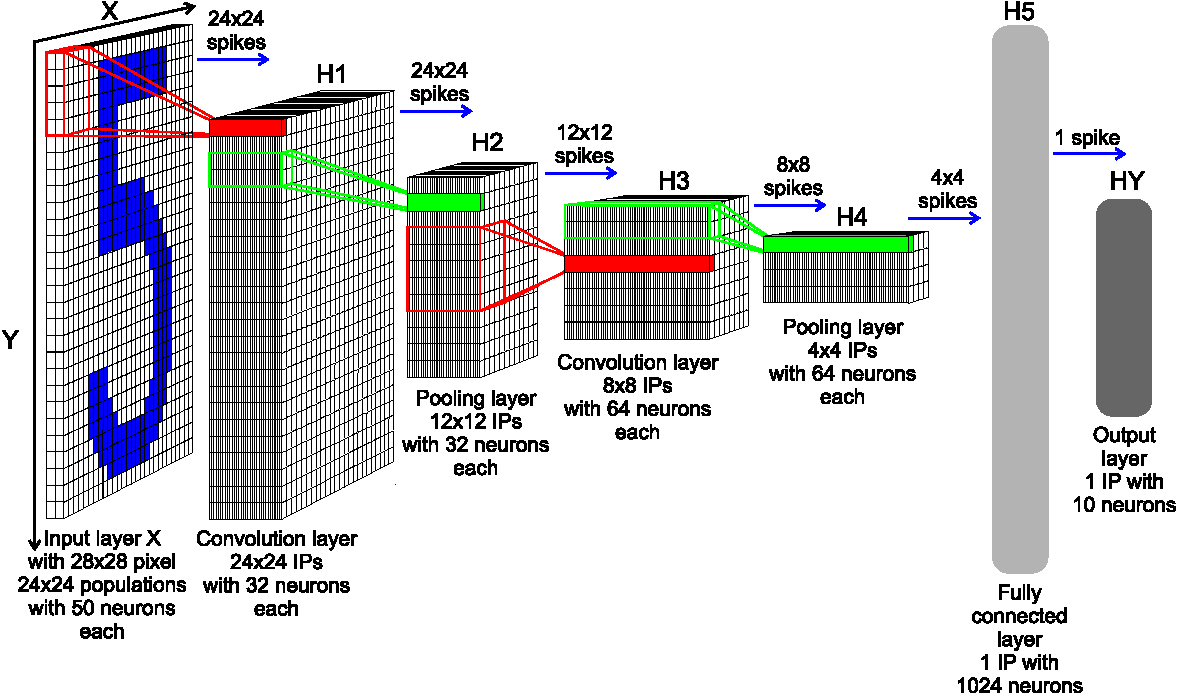
\includegraphics[width=0.5\columnwidth]{./chapters/sbs_accelerator/figures/sbs_network.pdf}
	\caption{\gls{sbs} network architecture for handwritten digit classification task.}
	\label{fig:sbs_network}
\end{figure*}


\begin{table}[t!]\centering
	\caption{\gls{sbs} network architecture for handwritten digit classification task.}
	\label{tab:sbs_network}
	\scriptsize
	\begin{tabular}{lrrrrrrr}\toprule
		&\multicolumn{3}{c}{\textbf{Layer size}} & &\multicolumn{2}{c}{\textbf{Kernel size}} \\\cmidrule{2-4}\cmidrule{6-7}
		\textbf{Layer} ($H^l$) &$N_X$ &$N_Y$ &$N_H$ & &$K_X$ &$K_Y$ \\\midrule
		Input ($HX$) &28 &28 &2 & &- &- \\
		Convolution ($H1$) &24 &24 &32 & &5 &5 \\
		Pooling ($H2$) &12 &12 &32 & &2 &2 \\
		Convolution ($H3$) &8 &8 &64 & &5 &5 \\
		Pooling ($H4$) &4 &4 &64 & &2 &2 \\
		Fully connected ($H5$) &1 &1 &1024 & &4 &4 \\
		Output ($HY$) &1 &1 &10 & &1 &1 \\
		\bottomrule
	\end{tabular}
\end{table}

\subsection{Computational Cost}

The number of \gls{mac} operations required for inference of an \gls{sbs} layer is defined by $NOPS_{MAC}=N_{Spk} N_X N_Y K_X K_Y (3 N_H + 2)$, where $N_{Spk}$ is the number of spikes (iterations), $N_X N_Y$ is the size of the layer, $K_X K_Y$ is the size of the kernel for convolution/pooling, and $N_H$ is the length of $\vec{h}$. The computational cost of \gls{sbs} network models is higher compared to equivalent \gls{cnn} models and lower compared to regular \gls{snn} models (e.g., \gls{lif}) \mbox{\cite{izhikevich2004model}}.


\begin{figure*}[b!]
	\centering
	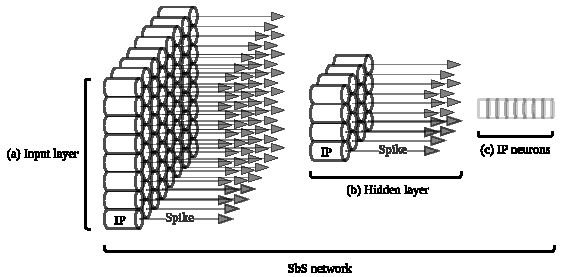
\includegraphics[width=0.5\columnwidth]{./chapters/sbs_accelerator/figures/SbS_layer.pdf}
	\caption{\gls{sbs} \glspl{ip_sbs} as independent computational entities, (a) illustrates an input layer with a massive amount of \glspl{ip_sbs} operating as independent computational entities, (b) shows a hidden layer with an arbitrary amount of \glspl{ip_sbs} as independent computational entities, (c) exhibits a set of neurons grouped in an \gls{ip_sbs}.}
	\label{fig:SbS_layer}
\end{figure*}


\subsection{Error Tolerance}

To illustrate the error tolerance of \gls{sbs} networks, it is presented a classification performance under positive additive uniformly distributed noise as external disturbance. \fig{fig:robustnes_sbs} presents a comparison of the classification performance of an \gls{sbs} network and a standard \gls{cnn}, with the same amount of
neurons per layer as well as the same layer structure. Both neural networks are trained for handwritten digit classification on MNIST dataset \cite{lecun1998mnist} (see \cite{rotermund2019Backpropagation} for details). The figure shows the correctness for the MNIST test set with its \num[group-separator={,}]{10000} patterns in dependency of the noise level for positive additive
uniformly distributed noise. The blue curve shows the performance for
the \gls{cnn}, while the red curve shows the performance for
the \gls{sbs} network with \num[group-separator={,}]{1200} spikes (iterations). Beginning
with a noise level of 0.1, the respective performances are different
with a p - level of at least $10^{-6}$ (tested with the Fisher exact
test). Increasing the number of spikes per \gls{sbs} population to \num[group-separator={,}]{6000}
(performance values shown as black stars), shows that more spikes can
improve the performance under noise even more.

\begin{figure*}[b!]
	\centering
	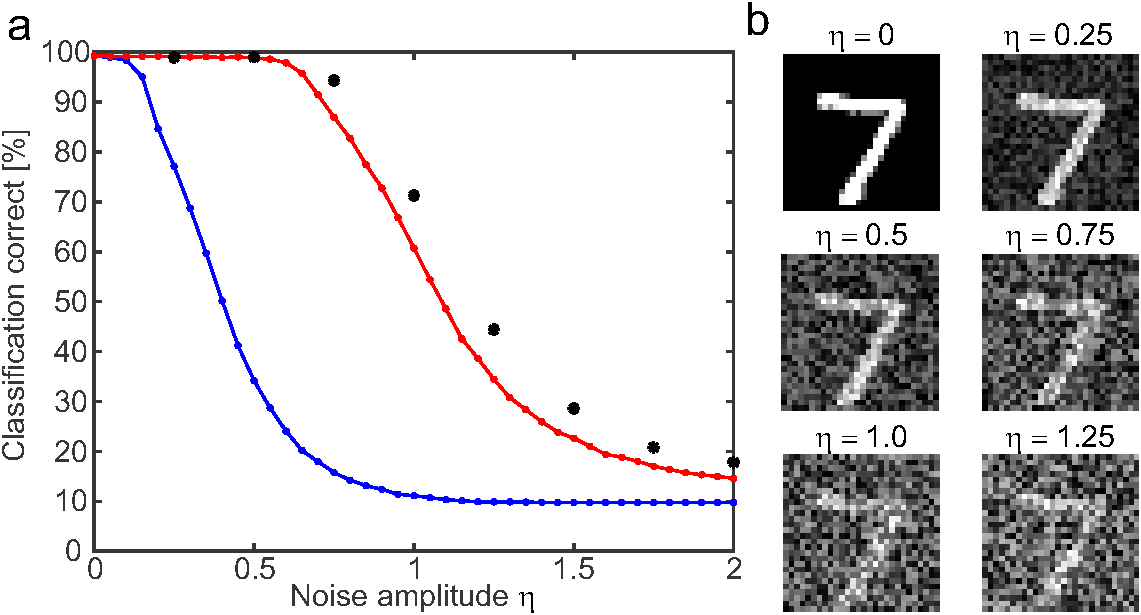
\includegraphics[width=0.5\columnwidth]{./chapters/sbs_accelerator/figures/sbs_robustnes.pdf}
	\caption{(a) Performance classification of \gls{sbs} NN versus equivalent \gls{cnn}, and (b) example of the first pattern in the MNIST test data set with different amounts of positive additive uniformly distributed noise.}
	\label{fig:robustnes_sbs}
\end{figure*}

%%%%%%%%%%%%%%%%%%%%%%%%%%%%%%%%%%%%%%%%%%%%%%%%%%%%%%%%%%%%%%%%%%%%%%%%%%%%%%%%%%%%%%
\section{Conv2D Tensor Operation}
A convolutional layer aims to learn and extract feature representations from an input. Each unit of a feature map is connected to a region of neighboring units on the input maps (from the previous layer). This neighborhood in the previous layer is known as the receptive field of such unit. A new feature map can be obtained by first convolving the input maps with a learned kernel and then applying a nonlinear elementwise activation function to the convolved results. All spatial locations on the input maps share a kernel to generate a feature map. All feature maps are obtained by convolving several different kernels~\cite{gu2018recent}.


The 2D convolution process is performed by the \emph{Conv2D} tensor operation, described in \Equ{eq:conv2D}, where $h$ is the input tensor containing the feature maps, $W$ is the convolution kernels (known as filters), and $b$ is the bias vector for the output feature maps~\cite{goodfellow2016deep}. $K\times L\times M$ is the receptive field size, $K\times L$ is the convolution kernel, and $M$ is the number of input channels/feature maps. In this work, the \emph{Conv} is denoted as \emph{Conv2D} operator.
\begin{eqnarray} \label{eq:conv2D}
Conv\left(W,h\right)_{i,j,o}=\sum_{k,l,m}^{K,L,M} h_{(i+k,j+l,m)} W_{(o,k,l,m)}+b_{o}
\end{eqnarray}

\section{Floating-point Number Representation}
The representation of every numerical value, in any numerical system, is made of an integer and a fractional part. The border that delimits them is called the radix point. The fixed-point format for representing numeric values derives its name from the fact that in this format, the base point is fixed at a certain position. For integer numbers, this position is at the right of the least significant digit.

In scientific computation, it is often necessary to represent very large and very small values. This is difficult to achieve using the fixed-point format because the bit size required to maintain both the desired precision and the desired range are very large. In such situations, \gls{fp} formats are used to represent real numbers. Each \gls{fp} number can be divided into three fields: sign $S$, exponent $E$, and mantissa $M$. Using the binary number system, it is possible to represent any \gls{fp} number as:

\begin{eqnarray} \label{eq:float}
(-1)^{S} \times 1.M \times 2^{E-B}
\end{eqnarray}

In \gls{fp} representations the exponent is biased. This bias depends on the bit size of the exponent field. This exponent bias is defined by \Equ{eq:float_bias}, where $E_{size}$ is the exponent bit size.

\begin{eqnarray} \label{eq:float_bias}
B=2^{E_{size}-1}-1
\end{eqnarray}

There is a natural trade-off between small bit size requiring fewer hardware resources and larger bit size providing higher precision. Within a given total bit size, it is possible to assign various combinations of sizes to the exponent and mantissa fields, with wider exponents resulting in a higher range and wider mantissa resulting in better precision.

The most widely used format for \gls{fp} arithmetic is the IEEE 754 standard \cite{zuras2008ieee}. The IEEE single-precision format (32-bit) is expressed by \Equ{eq:float} with $B$ = 127, 8 bits for the exponent and 23 bits for the mantissa, see \Fig{fig:floating}(a). In \gls{fp} formats, the numbers are normalized, the leading one is an implicit bit, and only the fractional part is explicitly stored in the mantissa field.

\begin{figure*}[b!]
	\centering
	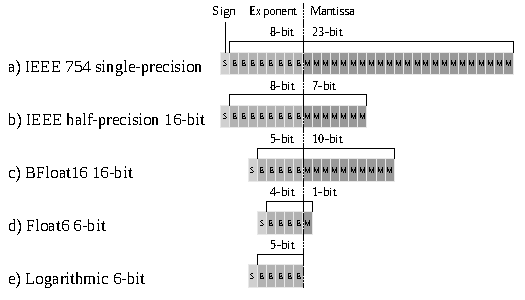
\includegraphics[width=0.5\columnwidth]{./chapters/cnn_accelerator/figures/power_breakdown/floating_point.pdf}
	\caption{Floating-point number representation.}
	\label{fig:floating}
\end{figure*}

Reduced bit size than those specified in the IEEE 754 standard are often sufficient to provide the desired precision. Reduced designs require fewer hardware resources enabling low-power implementations. In custom hardware designs, it is possible to customize the \gls{fp} format implemented. In later sections, the term E$a$M$b$ is used to denote \gls{fp} formats, where $a$ and $b$ are the exponent and mantissa bit size, respectively. For example, E4M1 means 4-bit exponent and 1-bit mantissa, see \Fig{fig:floating}(d).

There are three special definitions in IEEE 754 standard. The first is subnormal numbers when $E=0$, then \Equ{eq:float} is modified to \Equ{eq:float_subnorm}. Infinity and \gls{nan} are the other two special cases but are not used in our work.

\begin{eqnarray} \label{eq:float_subnorm}
(-1)^{S} \times 0.M \times 2^{1-B}
\end{eqnarray}